\documentclass[12pt,a4paper,final]{article}
\usepackage[utf8]{inputenc}
\usepackage{amsmath}
\usepackage{amsfonts}
\usepackage{amssymb}
\usepackage{graphicx}
\usepackage[margin=1in]{geometry}  
\usepackage{caption}
\usepackage{subcaption}
\begin{document}

\section*{Lab 2 Report}

\subsection*{Part 1 - Corner Detection}
Include one image with corners identified. 

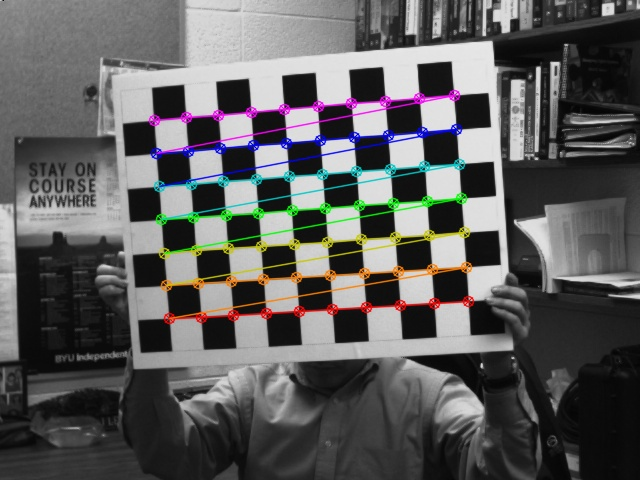
\includegraphics[scale=0.25]{Task_1}

\subsection*{Part 2 - Intrinsic Parameters}
Intrinsic Matrix:
\begin{equation*}
\begin{bmatrix}
1145.37 & 0 & 328.0 \\ 0 & 1143.77 & 222.23 \\ 0 & 0 & 1
\end{bmatrix}
\end{equation*}
Distortion Parameters:
\begin{equation*}
\begin{bmatrix}
-0.258 \\ 0.0423 \\ -0.0014 \\ -0.0014 \\1.746
\end{bmatrix}
\end{equation*}

\subsection*{Part 3 - Distortion Correction}
\begin{figure}[h]
\centering
\begin{subfigure}{.3\textwidth}
  \centering
  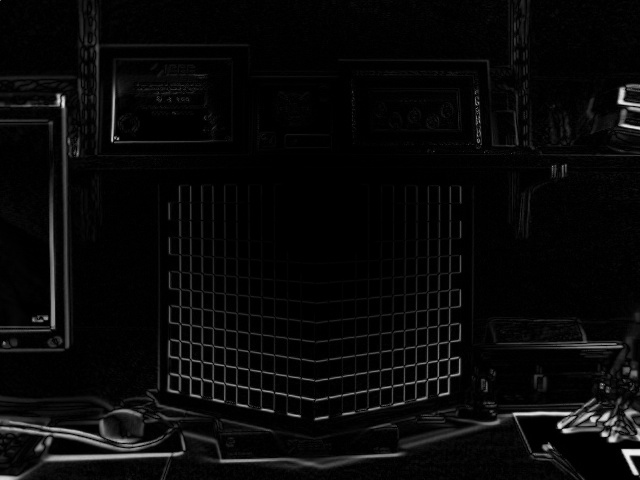
\includegraphics[width=.9\linewidth]{far_diff}
  \caption{Far diff}
  \label{fig:sub1}
\end{subfigure}%
\begin{subfigure}{.3\textwidth}
  \centering
  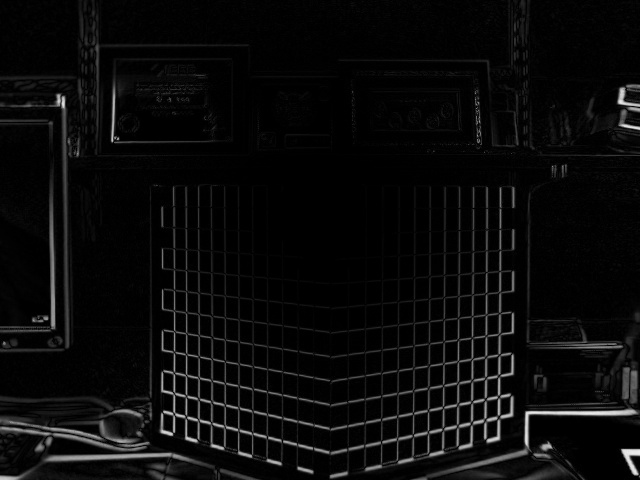
\includegraphics[width=.9\linewidth]{close_diff}
  \caption{Near diff}
  \label{fig:sub2}
\end{subfigure}
\begin{subfigure}{.3\textwidth}
  \centering
  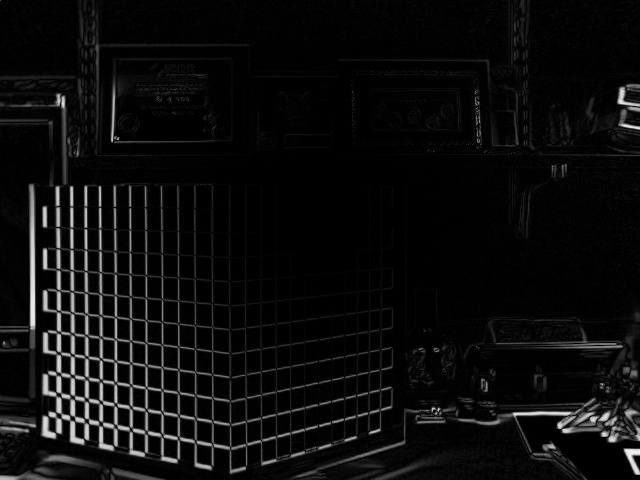
\includegraphics[width=.9\linewidth]{turned_diff}
  \caption{Turned diff}
  \label{fig:sub3}
\end{subfigure}
\label{fig:test}
\end{figure}

\subsection*{Part 4 - Object Pose Estimation}

Rotation Matrix:
\begin{equation*}
\begin{bmatrix}
0.5855 & 0.3246 & 0.7429 \\
  0.2130 & -0.9458 & 0.2453 \\
  0.7822 & 0.01461 & -0.6229
\end{bmatrix}
\end{equation*}
Translation Matrix:
\begin{equation*}
\begin{bmatrix}
-1.1785 \\ -0.4288 \\ -1.6175
\end{bmatrix}
\end{equation*}

\subsection*{Part 5 - Intrinsic Parameters}
Intrinsic Matrix:
\begin{equation*}
\begin{bmatrix}
1599.25 & 0 & 204.666\\ 0 & 1515.27 & 298.007\\ 0 & 0 & 1
\end{bmatrix}
\end{equation*}
Distortion Parameters:
\begin{equation*}
\begin{bmatrix}
0.03891 \\ 3.7005 \\ 0.0093\\ -0.0182 \\-45.8114
\end{bmatrix}
\end{equation*}

\subsection*{Part 6 - Distortion Correction}

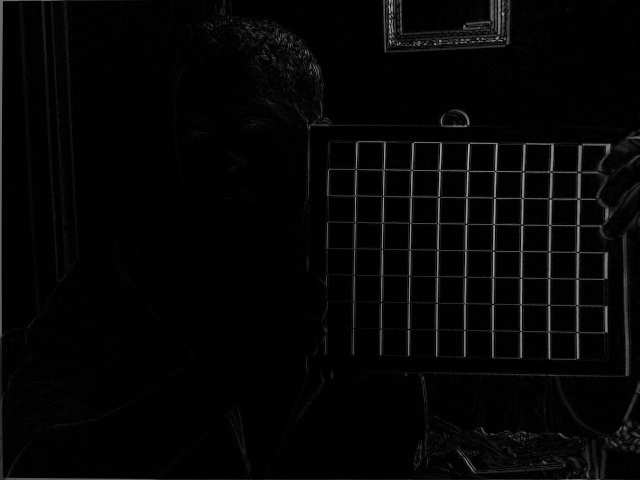
\includegraphics[scale=0.25]{webcam1}

\subsection*{Explanation}

The code provided in the assignment can all be made with the included CMakeLists.txt file. The images that are read in in task 2 need to be in a subdirectory named jpg\textunderscore calibration and named as in the jpeg folder off the website. The files Close.jpg, Far.jpg, object\textunderscore with\textunderscore corners.jpg, and Turned.jpg need to be in the same directory as the build executables. The executable names can be obtained from CMakeLists.txt. The intrinsic parameters file in part 5 requires you to press the spacebar each time you want to take a picture. When you are done acquiring images, press the 'x' key for processing to take place to produce intrinsic parameters. This file also requires the directory 'calibrate\textunderscore webcam' to be created and/or cleared beforehand (unless c++ automatically creates the appropriate directory)

\end{document}